\kommentar{Schwingkreise}

\begin{karte}{Wie verhält sich ein echter Kondensator?}
	Ein Kondensator ist laut dem Ersatzschaltbild ein Serienschwingkreis und hat dementsprechend folgenden Verlauf:
	
	\begin{minipage}{0.48\textwidth}
		\scalebox{.7}{%Autor: Simon Walker
%Version: 1.0
%Datum: 19.04.2020
%Lizenz: CC BY-NC-SA

\begin{circuitikz}
	%	\HelpCords{-1}{-1}{7}{1}
	
	\draw
	%Knoten
	(0, 0) coordinate (n1)
	(2, 0) coordinate (n2)
	(4, 0) coordinate (n3)
	(6, 0) coordinate (n4)
	
	%Nur zu Hilfszwecken
	%	(n1) node[above] {$n1$}
	%	(n2) node[above] {$n2$}
	%	(n3) node[above] {$n3$}
	%	(n4) node[above] {$n4$}
	
	(n1) to[C=$C$, o-] (n2) to [R=$R(\omega)$] (n3) 
	to [american inductor=$L$, -o] (n4)
	;
\end{circuitikz}
}
	\end{minipage}
	\begin{minipage}{0.48\textwidth}
		%Autor: Simon Walker
%Version: 1.0
%Datum: 19.04.2020
%Lizenz: CC BY-NC-SA

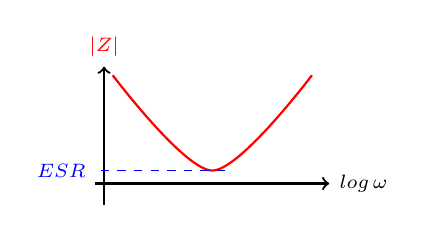
\begin{tikzpicture}[smooth, xscale=0.55, yscale=0.55]
	% Achsen
	\draw[->, thick] (-0.2,0) -- (5.2,0) node[right] {$\scriptstyle log \, \omega$}; % Horizontal
	\draw[->, thick] (0,-0.5) -- (0,2.7) node[above] {$ \scriptstyle \color{red} \left|Z\right|$}; % Vertikal
	
	%Impedanzfunktion
	\draw [red, thick] plot [smooth] coordinates{
		(0.2, 2.5) (2.5, 0.3) (4.8, 2.5)
	};

	%Beschriftungen
	\draw [blue, dashed] (2.8, 0.3) -- (-0.2, 0.3)
	node[left] {$\scriptstyle ESR$};
	
	
\end{tikzpicture}

	\end{minipage}\\[5pt]
	Das Minimum der Impedanzfunktion ist rein reell und wird ESR (Equivalent Series Resistance) genant. Es enspricht dem Wert des Seriewiderstands bei der entsprechenden Frequenz.
\end{karte}

\begin{karte}{Wie verhält sich ein echten Widerstand?}
	Das Ersatzschaltbild eines Widerstands hat entweder eine Spule in Serie (für  kleine $R$) oder einen Kondensator Parallel (für grosse $R$).
	
	\begin{minipage}{0.48\textwidth}
		\scalebox{.85}{%Autor: Simon Walker
%Version: 1.0
%Datum: 19.04.2020
%Lizenz: CC BY-NC-SA

\begin{circuitikz}
%	\HelpCords{-1}{-3}{5}{1}
	
	\draw
	%Knoten
	(0, -2) coordinate (n11)
	(1, -2) coordinate (n12)
	(1, -2.75) coordinate (n13)
	(1, -1.25) coordinate (n14)
	(3, -2.75) coordinate (n15)
	(3, -1.25) coordinate (n16)
	(3, -2) coordinate (n17)
	(4, -2) coordinate (n18)
	
	(0, 0) coordinate (n21)
	(2, 0) coordinate (n22)
	(4, 0) coordinate (n23)
	
	
	%Nur zu Hilfszwecken
%	(n11) node[above] {$n11$}
%	(n12) node[above] {$n12$}
%	(n13) node[above] {$n13$}
%	(n14) node[above] {$n14$}
%	(n15) node[above] {$n15$}
%	(n16) node[above] {$n16$}
%	(n17) node[above] {$n17$}
%	(n18) node[above] {$n18$}
	
%	(n21) node[above] {$n21$}
%	(n22) node[above] {$n22$}
%	(n23) node[above] {$n23$}
	;
	%Serie L
	\draw[red]
	(n21) to[R=$R$, o-, color=red] (n22) 
	to [american inductor=$L$, -o, color=red] (n23)
	;
	
	
	%Parallel C
	\draw[blue]
	(n11) to[short, o-*, color=blue] (n12)
	(n13) to[short, color=blue] (n14)
	(n14) to[R=$R$, color=blue] (n16)
	(n13) to[C=$C$, color=blue] (n15)
	(n16) to[short, color=blue] (n15)
	(n17) to[short, *-o, color=blue] (n18)
	;
\end{circuitikz}
}
	\end{minipage}
	\begin{minipage}{0.48\textwidth}
		%Autor: Simon Walker
%Version: 1.0
%Datum: 19.04.2020
%Lizenz: CC BY-NC-SA

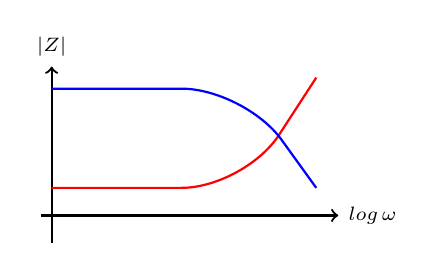
\begin{tikzpicture}[smooth, xscale=0.7, yscale=0.7]
	% Achsen
	\draw[->, thick] (-0.2,0) -- (5.2,0) node[right] {$\scriptstyle log \, \omega$}; % Horizontal
	\draw[->, thick] (0,-0.5) -- (0,2.7) node[above] {$ \scriptstyle \left|Z\right|$}; % Vertikal
	
	%Impedanzfunktion Serie (kleines R)
	\draw [red, thick, rounded corners=8mm] 
		(0, 0.5) -- (3.5, 0.5) -- (4.8, 2.5);
		
	%Impedanzfunktion Parallel (grosses R)
	\draw [blue, thick, rounded corners=8mm] 
	(0, 2.3) -- (3.5, 2.3) -- (4.8, 0.5);
	
\end{tikzpicture}

	\end{minipage}\\[5pt]
\end{karte}

\begin{karte}{Wie verhält sich eine echte Spule?}
	Das Ersatzschaltbild einer Spule ist ein Parallelschwingkreis. Deshalb hat der Impedanzverlauf folgende Eigenschaften.
	
	\begin{minipage}{0.48\textwidth}
		%Autor: Simon Walker
%Version: 1.0
%Datum: 19.04.2020
%Lizenz: CC BY-NC-SA

\begin{circuitikz}
%	\HelpCords{-1}{-1}{5}{1}
	
	\draw
	%Knoten
	(0, 0) coordinate (n1)
	(1, 0) coordinate (n2)
	(1, -0.75) coordinate (n3)
	(1, 0.75) coordinate (n4)
	(3, -0.75) coordinate (n5)
	(3, 0.75) coordinate (n6)
	(3, 0) coordinate (n7)
	(4, 0) coordinate (n8)
	
	
	%Nur zu Hilfszwecken
%	(n1) node[above] {$n1$}
%	(n2) node[above] {$n2$}
%	(n3) node[above] {$n3$}
%	(n4) node[above] {$n4$}
%	(n5) node[above] {$n5$}
%	(n6) node[above] {$n6$}
%	(n7) node[above] {$n7$}
%	(n8) node[above] {$n8$}
	
	;	


	\draw
	(n1) to[short, o-*] (n2)
	(n3) to[short] (n4)
	(n4) to[american inductor=$L$] (n6)
	(n3) to[C=$C$] (n5)
	(n6) to[short] (n5)
	(n7) to[short, *-o] (n8)
	;
\end{circuitikz}

	\end{minipage}
	\begin{minipage}{0.48\textwidth}
		%Autor: Simon Walker
%Version: 1.0
%Datum: 19.04.2020
%Lizenz: CC BY-NC-SA

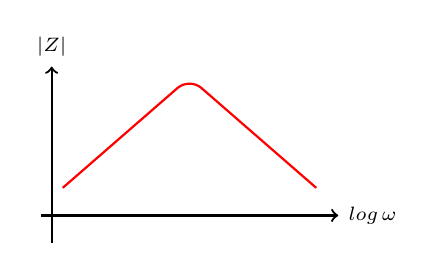
\begin{tikzpicture}[smooth, xscale=0.7, yscale=0.7]
	% Achsen
	\draw[->, thick] (-0.2,0) -- (5.2,0) node[right] {$\scriptstyle log \, \omega$}; % Horizontal
	\draw[->, thick] (0,-0.5) -- (0,2.7) node[above] {$ \scriptstyle \left|Z\right|$}; % Vertikal
	
		%Impedanzfunktion
	\draw [red, thick, rounded corners=2mm] 
		(0.2, 0.5) -- (2.5, 2.5) -- (4.8, 0.5);
	
\end{tikzpicture}

	\end{minipage}\\[5pt]
\end{karte}
